\chapter{Ground state}
\label{chap:ground}

From the ground state of the model hamiltonian (\ref{eq:full-hamiltonian}) we can calculate, using (\ref{eq:dvsuir}), the split CuO distance for different values of the coupling parameter $\lambda_{ir}$.
In section \ref{sec:grd-phonon-proj} of this chapter we reproduce the previous work by Mustre de Le\'{o}n \textit{et al.} \cite{MustredeLeon1992} which, from this calculation, determied that the relevant couplings are in the intermediate regime.

Since the model hamiltonian (\ref{eq:full-hamiltonian}) exhibits polaronic behaviour only for electron-lattice couplings greater than zero, we can identify the difference between the ground state energy in the absence of electron-lattice interaction ($\lambda_{ir}=0$) and its value for the coupling value where this polaronic behaviour sets in as the bipolaron binding enerygy.
In section \ref{sec:grd-binding-energy} we calculate this binding energy comparing it with experimental results.
We also calculate the isotopic shift, as defined in (\ref{eq:isot-shift-def-grd}), for the oxygen substitution$^{16}$O$\rightarrow ^{18}$O as a function of $\lambda_{ir}$.

\section{Projection into phonon coordinates}
\label{sec:grd-phonon-proj}

% Split distance discussion

\begin{figure}[ht!]
  \centering
  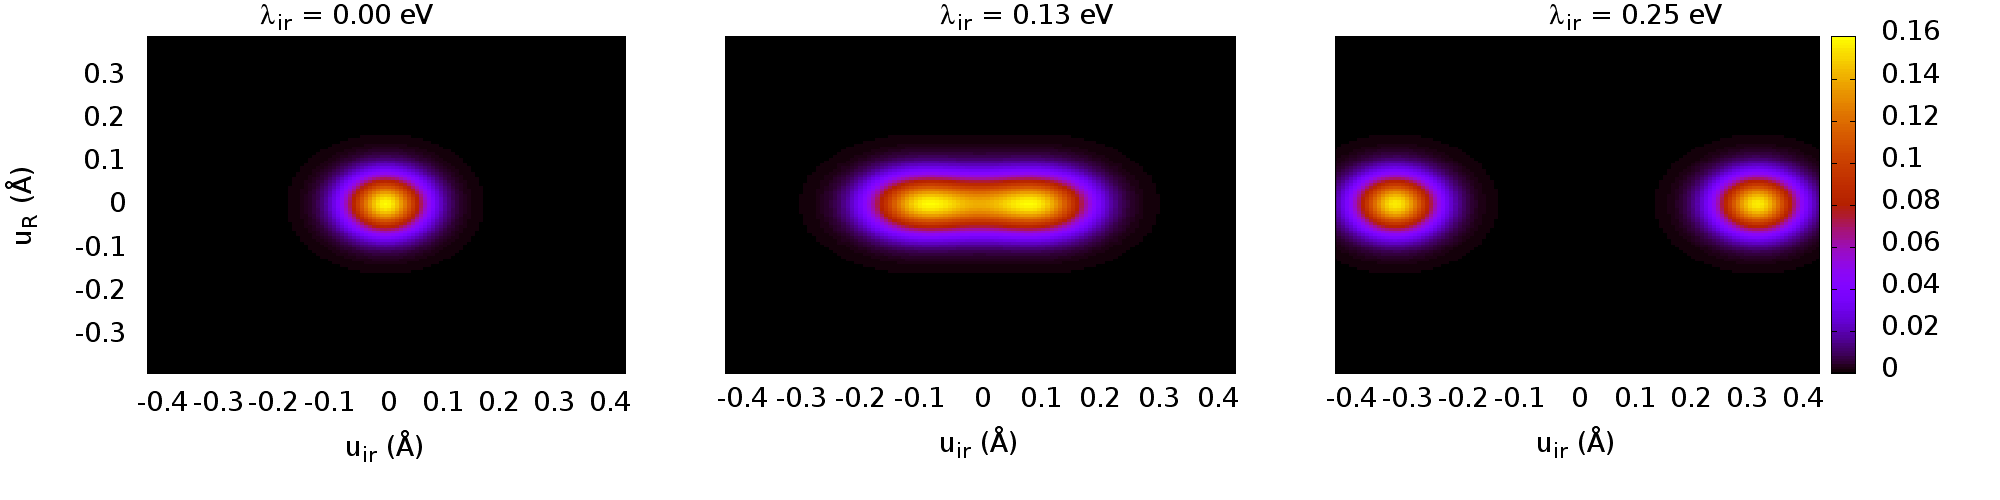
\includegraphics[width=1.0\textwidth]{images/ph-ground.png}
  \caption{Ground state's projection into phonon coordinates for three different values of the coupling parameter $\lambda_{ir}$.}
  \label{fig:ph-ground}
\end{figure}

\section{Bipolaron binding energy}
\label{sec:grd-binding-energy}

The bipolaron formation energy is $E_p = E(\lambda_{ir}=0)- E(\lambda_{ir}=0.13$ eV$) \sim 42$ meV and corresponds to the bipolaron binding energy. This value compares favorably with the value obtained from femtosecond time-domain spectroscopy ($E_p \sim 45$ meV for YBa$_2$Cu$_3$O$_7$ \cite{Demsar1999}. We also find that if we consider a smaller electron-lattice coupling such that the distortion is 0.08 $\AA$, as that observed for in plane Cu(2)-O in La$_{1.85}$Sr$_{0.15}$CuO$_4$ \cite{Bianconi1996}, we obtain $E_p \sim 32$ meV, which is also comparable to estimates for the pseudogap formation energy in this system \cite{Kusar2005}.


For the ground state we define the energy isotopic shift $\Delta_g$ in a similar way but with the energies measured relative to the uncoupled system (that is, the system with $\lambda_{ir}=\lambda_R=0$) (see \ref{isot-shift-def-grd}):

\begin{equation}
  \Delta_g = \frac{\Delta E_g(^{16}O)- \Delta E_g(^{18}O)}{\Delta E_g(^{16}O)} \times 100 
\end{equation}

where $\Delta E_g \equiv E_g - E_g(\lambda_{ir}=0, \lambda_R=0)$. To calculate this energies we need to take into account the *zero-point energy* in the phononic part $H_{ph}$ from (\ref{eq:full-hamiltonian}) writting it as \ref{phononic-part-complete}

The following figure plots this isotopic shift:

\begin{figure}[ht!]
  \centering
  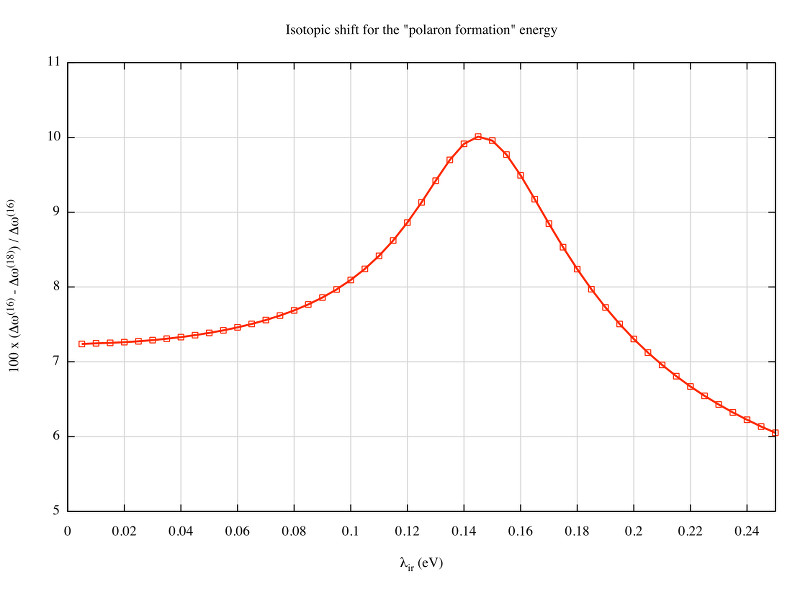
\includegraphics[width=0.8\textwidth]{images/isot_polaron_formation.jpg}
  \caption{Isotopic shift of the polaron formation energy.}
  \label{fig:isot_polaron_formation}
\end{figure}

Although $\Delta_g$ doesn't change sign, as the isotopic shift of the polaron tunneling state, it shows a maximum in the middle coupling regime reminiscent of the maximums, minimums or inflection points in the isotopic shifts for all the other excitations.